% !TEX root = ../CINTA-cn.tex
%%%%%%%%%%%%%%%%%%%%%%%%%%%%%%%%%%%%%%%%%%%%%%%%%%%%%%%%%%%%%%%%%%%%
% Author: Libin Wang
% Chapter 15. DLOG
% This document was released as open source on 2026-06-18.
% Copyright 2023, Libin Wang. Creative Commons License
% This work is licensed under a Creative Commons Attribution-NonCommercial-NoDerivatives 4.0 International License.
%%%%%%%%%%%%%%%%%%%%%%%%%%%%%%%%%%%%%%%%%%%%%%%%%%%%%%%%%%%%%%%%%%%%
\chapter{离散对数}
\label{chap:dlog} 
\begin{introduction}
  \item 离散对数问题
  \item Pohlig-Hellman 算法
  \item 大步小步算法
  \item  Rho 算法
\end{introduction}
\section{引言}
\label{sec:intro_dlp}
本章讨论求离散对数的算法，先看定义。

\begin{definition}{离散对数问题}{dlp}
	设$\mathbb{G}$为群，给定任意元素$g\in \mathbb{G}$（不要求$g$为群$\mathbb{G}$的生成元）和$y\in \langle g \rangle$。
	所谓\emph{离散对数问题}（\emph{discrete logarithm problem}，简记为 DLP ）
	即要计算$x$使得$g^x = y$。称解$x$为$y$以$g$为基底的离散对数值。
\end{definition}

以上定义不要求$g$为群$\mathbb{G}$的生成元，这使得离散对数问题的定义更具有普遍意义。实际应用中，我们也确实需要
在某些非循环群中求离散对数，比如第~\ref{chap:EC}章的椭圆曲线群。也有教科书或者科技论文要求基底$g$为群的生成元，
这个要求并不影响以下算法的计算。

首先，我们知道，求连续型对数是容易的。即，在实数域上，给定$y = \log_g \; x$，求$x$是容易的。
图~\ref{fig:clog}展示在$g = 2$时，$x$与$y$之间存在某种直观的规律关系，而这种关系直接导致求连续型对数的易解。
\begin{figure}
\begin{center}
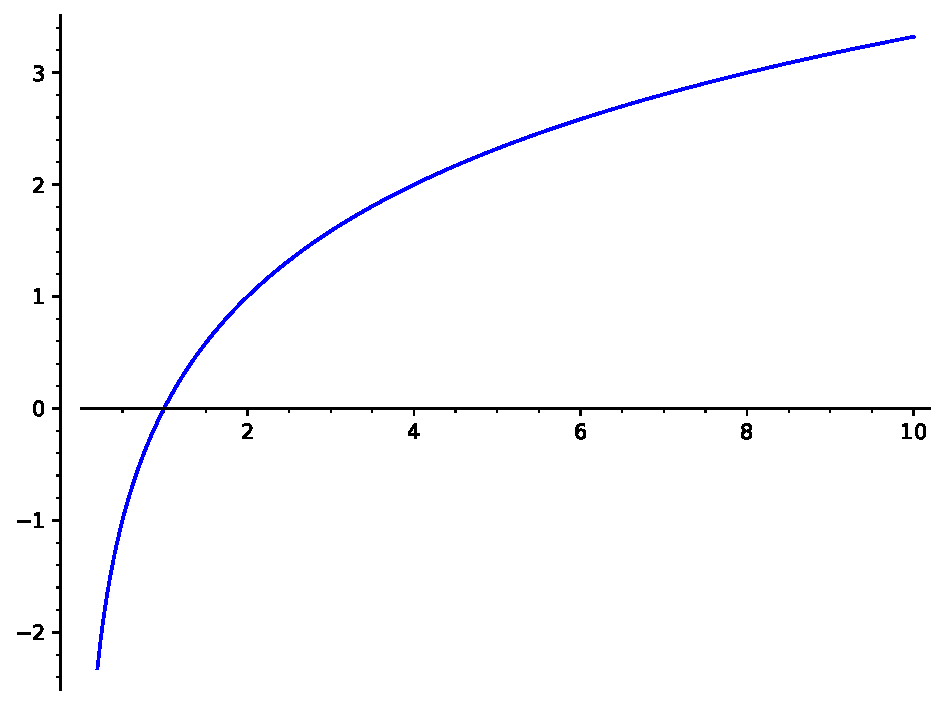
\includegraphics[width=0.6\textwidth]{figures/chapt15-1-continuous-logarithm.pdf} 	
\caption{连续型对数函数$y = \log_2 \; x$。}
\label{fig:clog}       % Give a unique label
\end{center}
\end{figure}

我们猜想，对给定$g$，如果$g^i$也满足某种规律，那么也许可以利用这种规律去寻找高效的求解方法。图~\ref{fig:dlog}
则显示出$\Z_p^*$群中的$g^i$呈现出一种均匀离散分布性，至少看上去如此。而这就是为什么某些 DLP 问题很难的部分原因。

\begin{figure}
\begin{center}
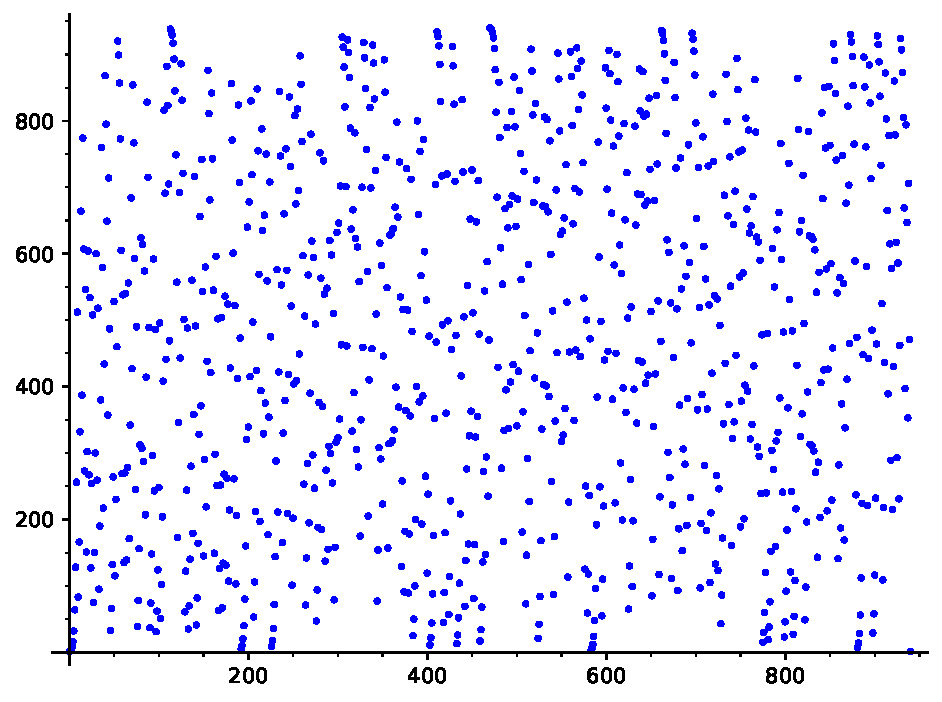
\includegraphics[width=0.75\textwidth]{figures/chapt15-2-discrete-logarithm-distribution.pdf} 	
\caption{$g = 2, p = 941$时$g^x \pmod{p}$的点集.}
\label{fig:dlog}       % Give a unique label
\end{center}
\end{figure}

穷举法是求离散对数问题的最朴素方法。容易想到，已知$g$和$y$，对变量$x$进行迭代计算，求$g^x$并判断它是否等于$y$，如果是，则$x$就是解。
显然，如果群$\mathbb{G}$很大，这种方法并不高效。
例如，给定一个长为$\lambda$比特的素数$p$，群$\Z_p^*$的大小是$p-1$，是$\mathcal{O}(2^{\lambda})$的规模。穷举法求离散对数
则需要$\mathcal{O}(2^{\lambda})$次乘法，是一种指数式的效率。当然，我们需要试图寻求更好的解决办法。

\section{Pohlig-Hellman 算法}
\label{sec:pha}
Pohlig-Hellman 算法是一种特殊的分治法，把一个 DLP 问题实例分解为若干个小的 DLP 问题，通过对小问题进行求解，
从而得到得目标问题的解。

考虑任意群$\mathbb{G}$，给定基底$g\in \mathbb{G}$，且$g$的阶为$n\in \N$，DLP 实例是$y = g^x$，目标
是计算出$x$。如果读者感觉把这里的任意群$\mathbb{G}$实例化为乘法群$\Z_p^*$更容易理解，也可以如此操作。
算法分为以下步骤：

\begin{enumerate}
\item 首先对$n$进行整数分解，即求得$n = p_1^{k_1} p_2^{k_2} \cdots p_t^{k_t}$，所有的$p_i$都是素数；

\item 令$g_i = (g^{n/p_i^{k_i}})$，$y_i = y^{n/p_i^{k_i}} $，得到了$t$个小的 DLP 问题的实例，
因为此时对所有的$0 \leq i \leq t$，$g_i^x = y_i$。

\item 对以上 DLP 实例进行求解，得到$t$个解$x_i$，$0 \leq i \leq t$；

\item  任意一个$g_i^x  = y_i$的解$x_i$与目标问题的解$x$满足以下关系：
\[ x \equiv x_i \pmod{p_i^{k_i}}\]
\noindent 因此，得到$t$个同余方程$x \equiv x_i \pmod{p_i^{k_i}}$，借助CRT可求出$x$。
\end{enumerate} 
	
以上算法的正确性稍后给出，先看具体算法执行过程和小数值实例。算法可表示为如下代码：
\begin{center}
	\lstinputlisting[label = alg:Pohlig-Hellman, caption = Pohlig-Hellman 算法.]{codes/PohHelDLP.py}
\end{center}

\begin{example}
设$p=131$，$g = 2$是$\Z_p^*$的生成元，给定$y = 80$，求$x$使得$y = g^x$。%x=50
首先，分解$p -1 = 2 \cdot 5 \cdot 13$。
第二步，因为$g$的阶是$130$，求得以下三个小的 DLP 问题实例：
\begin{align*}
(g^{130/13})^x &\equiv y^{130/13} \pmod{131}\\
(g^{130/5})^x &\equiv y^{130/5} \pmod{131}\\
(g^{130/2})^x &\equiv y^{130/2} \pmod{131}
\end{align*}
代入$g$和$y$并计算可得：
\begin{align*}
 107^x &\equiv 63 \pmod{131}\\
 53^x &\equiv 1 \pmod{131}\\
 130^x &\equiv 1 \pmod{131}
\end{align*}

第三步，计算以上 DLP 实例，得到：
\begin{align*}
 x_1 &\equiv  11 \pmod{13}\\
 x_2 &\equiv 0 \pmod{5}\\
 x_3 &\equiv  0 \pmod{2}
\end{align*}

最后，对以上同余方程组运用CRT，求得$x = 50$。

可以使用 SageMath 验证以上计算。
\begin{lstlisting}
sage: p = 131
sage: g = Mod(2, p)  #表示g是模p下的值
sage: y = g^50            #因此，所有与g相关的计算都模p
sage: discrete_log(y, g, p)
50
\end{lstlisting}

\end{example}

\noindent \textbf{算法的正确性.} 要证明算法的正确性，需要证明以下两个性质。

第一点，所构造出的小 DLP 实例确实是以$g_i$为基底、离散对数值是目标问题的离散对数值，即$g_i^x = y_i$成立。
因为$g^x = y$，所以对任意$0 \leq i \leq t$
\[g_i^{x} = (g^{n/p_i^{k_i}})^x = (g^x)^{n/p_i^{k_i}} = y^{n/p_i^{k_i}} = y_i\]
即$g_i^x  = y_i$。

第二点，要证明任意一个$g_i^x  = y_i$的解$x_i$与目标问题的解$x$满足关系$x \equiv x_i \pmod{p_i^{k_i}}$，只
需要证明任意一个$g_i$的阶是$p_i^{k_i}$。首先要注意到
\[g_i^{p_i^{k_i}} = (g^{n/p_i^{k_i}})^{p_i^{k_i}} = g^n = 1 \]
即$g_i$的阶整除$p_i^{k_i}$。假设$g_i$的阶是$p_i^{k_i'}$，$k_i' \leq k_i$。则有：
\[g_i^{p_i^{k_i'}} =  g^{(n/p_i^{k_i})p_i^{k_i'}} = g^{n/p_i^{k_i - k_i'}} = 1\]
因为$g$的阶是$n$，所以，只能是$k_i' = k_i$，即$g_i$的阶就是$p_i^{k_i}$。

\noindent \textbf{算法的复杂性.}
Pohlig-Hellman 算法的计算主要包括三部分：分解基底$g$的阶$n$；求解$t$个小的 DLP 问题；计算 CRT 问题。大整数分解是难题，
这个问题在第~\ref{chap:factoring}章详细讨论，所以，Pohlig-Hellman 算法通常是假设$n$的素因子已知的情况下进行 DLP 求解。
求解 CRT 问题是容易的，请参考第~\ref{chap:crt}的结论。比较奇怪的是在求解 DLP 问题的时候借助了 DLP 问题的求解算法。
其实，这在算法理论当中是常见的手段。读者在此需要体会的是，构造出的所有 DLP 问题实例$g_i^x  = y_i$确实是更“小”的问题。
这种小体现在$g_i$的阶变小了，从某个$n$变成了某个$p_i^{k_i}$。即使从最肤浅的层面看，阶变小了，穷举都会变容易很多。
当然，实际上我们还可以借助下面章节的算法得到更好的效率。

会不会某些$n$的素因子还是足够大，使得相应的 DLP 问题求解依然很难呢？当然有这种情况。所以，综上所述，Pohlig-Hellman 算法
并不是一种高效的 DLP 求解方法，但是为 DLP 问题求解提供了一种可供参考的研究思路。

\section{大步小步算法}
\label{sec:bsgs}
以下这种称为
\emph{大步小步算法}（\emph{baby-step/giant-step algorithm}，简记为 BSGS）
\index{大步小步算法}\index{baby-step/giant-step algorithm}
的 DLP 求解算法是一种通过牺牲存储来换取效率的方法，思路很简单：通过两种不同的计算方式得到两个形式不同但是值相同的群元素，
从而算出离散对数值。

对任意的群$\mathbb{G}$，选取$g \in \mathbb{G}$，设$g$的阶为$p$，DLP 实例是$g^x = y$。算法过程如下：
\begin{itemize}
\item 大步过程:  将群$\mathbb{G}$分割成若干部分，每部分之间的区间大小为$s = \lfloor \sqrt{p} \rfloor$。具体计算如下：
\[ g^0, g^s, g^{2s}, \ldots , g^{\lfloor p/s \rfloor \cdot s} \]

\item 小步过程: $y$必然落在某个区间，即存在某个$t$使得$y$落在$g^{(t-1)s}$与$g^{ts} $之间。因此，计算：
\[y\cdot g, y\cdot g^2, \ldots, y\cdot g^s\]

\item 将以上计算结果分别存储，通过搜索发现如果存在某个$r$和某个$t$使得$y \cdot g^r = g^{t s}$，此时也称两种不同的计算
发生了一次\emph{碰撞}（\emph{collision}）。
于是$x = (ts - r) \pmod{p}$，简单计算可得$x$。
\end{itemize}

图~\ref{fig:bsgs}展示了 BSGS 算法的直观思路。图中上层标识了大步过程的群分割，下层标识小步过程的逼近计算。
可能需要强调，这个图是为了展示算法的直观，实际上每一个区间并不是连续的而是离散的点集，$g^{rs}$也不是按顺序排列的值。

\begin{thinking}
  读者有没有发现图~\ref{fig:bsgs}与图~\ref{fig:division}很相似？它们是在表达类似的思路吗？
\end{thinking}

具体算法展示如下。
\begin{figure}
\begin{center}
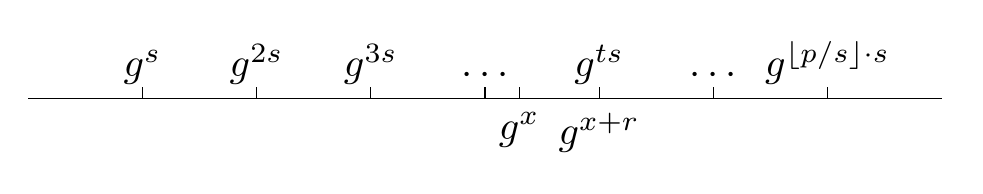
\begin{tikzpicture}[scale=1.45, transform shape]

\coordinate (A) at (1, 0);
\coordinate (B) at (2, 0);
\coordinate (C) at (3, 0);
\coordinate (D) at (4, 0);
\coordinate (E) at (5, 0);
\coordinate (F) at (6, 0);
\coordinate (G) at (7, 0);
\coordinate (H) at (8, 0);
\coordinate (I) at (9, 0);

\coordinate (K) at (5.3, 0);

\draw[-] (A)--(I) node {};

\draw (B) node[above] {$g^s$} -- ++(0, 3pt);
\draw (C) node[above] {$g^{2s}$} -- ++(0, 3pt);
\draw (D) node[above] {$g^{3s}$} -- ++(0, 3pt);
\draw (E) node[above] {$\cdots$} -- ++(0, 3pt);
\draw (F) node[above] {$g^{ts}$} -- ++(0, 3pt);
\draw (F) node[below] {$g^{x+r}$} -- ++(0, 3pt);
\draw (G) node[above] {$\cdots$} -- ++(0, 3pt);
\draw (H) node[above] {$g^{\lfloor p/s \rfloor \cdot s}$} -- ++(0, 3pt);
\draw (K) node[below] {$g^x$} -- ++(0, 3pt);

\end{tikzpicture}

\caption{BSGS 算法的几何解释.}
\label{fig:bsgs}       % Give a unique label
\end{center}
\end{figure}

\begin{center}
	\lstinputlisting[label = alg:bsgs, caption = 大步小步算法.]{codes/BGS-DLP.py}
\end{center}

\begin{example}
设群为$\Z_p^*$，$p = 37$，设$g = 2$，$y = 15$，求$x$使得$g^x = y$。首先，$s = \lfloor \sqrt{p} \rfloor = 6$
大步过程计算：
\[g^s = 27, g^{2s}=26 ,  g^{3s}=36 , g^{4s}=10 , g^{5s}=11 , g^{6s}= 1 \]
小步过程计算：
\[y\cdot g^1 =30 , y\cdot g^2 =23,  y\cdot g^3 = 9, y\cdot g^4=18,  y\cdot g^5=36, y\cdot g^s =35, \]
观察可知，$g^{3s} = y\cdot g^5$，即$t = 3$，$r = 5$，计算$x = (ts - r) \pmod{p} = 13$。用 SageMath 验证计算结果。

\begin{lstlisting}
sage: p = 37
sage: g = Mod(2, p)       #表示g是模p下的值
sage: y = g^13                #因此，所有与g相关的计算都模p
sage: bsgs(g, y, (0,p)) #这里要求提供的是一个区间
13
\end{lstlisting}
%bsgs(g,y,(0, p))
\end{example}
BSGS 算法的正确性主要体现在大步过程与小步过程所得计算结果必然会发生碰撞。图~\ref{fig:bsgs}已经做了很好的说明，
其实质就是除法算法。BSGS 算法的计算开销重点包括：大步、小步过程，分别是$\mathcal{O}(\sqrt{p})$次群乘法；排序与搜索
的开销是$\mathcal{O}(\sqrt{p} \log\; \sqrt{p})$。所以，BSGS 算法的复杂性就是$\mathcal{O}(\sqrt{p} \log\; p)$。

\section{Rho 算法}
\label{sec:prho}
Rho 算法与 BSGS 算法有类似的之处，都是希望通过计算出两个形式不同但是值相同的群元素，即通过找到碰撞来求解 DLP。
Rho 算法不同于 BSGS 算法，它并不存储大量的数据，而是通过两个不同的随机计算过程（理论上称为随机游动）来寻找碰撞。
这是一种通用的思路，也可以用于分解大整数，正如我们在第~\ref{chap:factoring}章看到的。

与之前一样，考虑任意的群$\mathbb{G}$，选取$g \in \mathbb{G}$，设$g$的阶为$q$，DLP 实例是$g^x = y$。
算法过程是一次“龟兔赛跑”过程：
\begin{enumerate}
\item 设定一个随机函数$f$，给定初始值$lg, ly, rg, ry \in \N$，这些值也称为指标值。计算$left = g^{lg} y^{ly}$和$right = g^{rg} y^{ry}$。
左值$left$扮演乌龟的角色，右值$right$扮演兔子的角色。

\item 迭代做以下计算：左值$left$（乌龟）进行一次慢计算$left =f(left)$，右值$right$（兔子）进行一次
快计算$right = f(f(right))$。
所谓“快计算”指的是它比“慢计算”多做了一次随机函数$f$的求值。注意，随机函数$f$的计算
除了更新$left$和$right$之外，还要同步更新$lg, ly, rg, ry$等指标值。

\item 如果在某个时刻左值与右值发生碰撞，即$left = right$，则$x = (lg - rg) / (ry - ly)$。
\end{enumerate} 

\begin{center}
	\lstinputlisting[label = alg:rho-dlog, caption = Rho 算法.]{codes/PollardRhoDLOG.py}
\end{center}

Rho 算法的过程写成代码如算法~\ref{alg:rho-dlog}所示，其中，为了方便，设$g$的阶为素数，读者能看出原因吗？
随机函数$f$的设定是算法的关键，Rho 算法的发明者 Pollard 建议使用以下函数：
\[ f(a) = \left \{
\begin{array}{ll}
ga & \text{如果}    \quad 0 \le a \leq \vert \mathbb{G} \vert /3, \\
a^2 & \text{如果} \quad \vert \mathbb{G} \vert /3 \leq a < 2\vert \mathbb{G} \vert /3,\\
ya & \text{如果}   \quad  2\vert \mathbb{G} \vert /3 \le a \le \vert \mathbb{G} \vert .
\end{array}
\right.
\]
 
如果$f$设定如上，则指标值$lg, ly$的更新如下所示，$rg, ry$的更新类似。
\[ f(lg) = \left \{
\begin{array}{ll}
lg + 1 & \text{如果} \quad 0 \le a \leq \vert \mathbb{G} \vert /3, \\
2 lg & \text{如果} \quad \vert \mathbb{G} \vert /3 \leq a < 2\vert \mathbb{G} \vert /3,\\
lg & \text{如果} \quad  2\vert \mathbb{G} \vert /3 \le a \le \vert \mathbb{G} \vert .
\end{array}
\right.
\]

\[ f(ly) = \left \{
\begin{array}{ll}
ly & \text{如果} \quad 0 \le a \leq \vert \mathbb{G} \vert /3, \\
2 ly & \text{如果} \quad \vert \mathbb{G} \vert /3 \leq a < 2\vert \mathbb{G} \vert /3,\\
ly + 1 & \text{如果} \quad  2\vert \mathbb{G} \vert /3 \le a \le \vert \mathbb{G} \vert .
\end{array}
\right.
\]
需要指出，以上随机函数及其相关更新规则的设定不具通用性，对于特定的群应该考虑做某些相应的改变。
\begin{example}
设$q = 23$，$p = 2 \cdot q + 1 = 47$，都是素数。令$a = 5$，这是$\Z_q^*$的生成元，令$g = a^2 = 25$，则
$g$是一个阶为$q$的群元。令$y = g^x  = 16$是 DLP 实例。请读者留意这里参数设定的含义。
初始指标值$lg = 1, ly = 0, rg = 0, ry = 1$，即$left = g = 25$，$right = y = 16$。

\noindent \textbf{乌龟过程：}
\begin{enumerate}
\item $left  = left \cdot g  = 14$， $lg = 2, ly = 0$

\item $left  = left \cdot g  = 21$，$lg = 3, ly =0$

\item $left  = left \cdot left = 18$，$lg = 6, ly =0$
\end{enumerate}

\noindent \textbf{兔子过程：}
\begin{enumerate}
\item $right = 18$, $rg = 0, ry = 4$

\item $right = 14$, $rg = 0, ry = 9$

\item $right = 18$, $rg = 2, ry =18$
\end{enumerate}

乌龟跑了三步，兔子其实是跑了六步，所以以上兔子的一步其实是两步，具体每一步的细节就不再详细列出，读者可以自行验证。
到了算法第三次迭代，发现$left = right$，非常幸运。
而且更幸运的是，$x = (lg - rg)/(ry - ly) = (6 - 2)/(18 - 0) $，在模$q$的意义下
求得$x = 13$。
\end{example}

Rho 算法的分析不再次展开，能成功求解离散对数问题的概率就是碰撞发生的概率，根据生日悖论，
碰撞发生的期望计算步骤是$\Theta(\sqrt{q})$，这就是 Rho 算法的复杂度。

%%2023年2月13日写
%%2023年6月24日
 \section*{章注}
 %\section*{Chapter Note}
 \addcontentsline{toc}{section}{章注}
不同群中的离散对数问题的难度并不相同。首先，需要避免一种误解，并非所有群的 DLP 都是难题。比如，如果求加法群$\Z_p$的离散对数问题，即给定$y \equiv x g \pmod{p}$求$x$，其中$y, g \in \Z_p$。
我们只需要使用欧几里得算法求$g$模$p$的乘法逆元。所以，求加法群的离散对数问题只需要线性时间。
而目前求解群$\Z_p^*$中的 DLP 最好的通用算法的效率是亚指数，比如使用 index calculus 算法。
求解第~\ref{chap:EC}章讲解的椭圆曲线群中的 DLP 更难，目前依然只有指数时间算法。

离散对数问题的难解性是 Diffie-Hellman 算法安全的基础，在实际应用中，如何确保所构造的群使得离散对数问题具有难解性，这一直是密码学家
长期关注的重点问题。

 \begin{problemset}
 \item 本题要求读者重新证明 Pohlig-Hellman 算法的正确性，但是要求有所降低，
 旨在让读者通过简单的实例去体会 Pohlig-Hellman 算法的发现思路。
 给定素数$p$，满足$(p - 1 )= p_1 p_2$，即$p-1$只有两个素因子。请证明针对$\Z_p^*$群，
 Pohlig-Hellman 算法能正确求解离散对数问题。
 
 \item 请用 Pohlig-Hellman 算法解决以下$\Z_p^*$群中的离散对数问题：
 \begin{enumerate}
 \item $p=71$，$g = 7$, $y = 53$；%ans. 23
 
 \item $p = 433$，$g = 5$，$y = 392$；%ans. 100
 \end{enumerate}
 
  \item 请用 BSGS 算法解决以下$\Z_p^*$群中的离散对数问题：
  \begin{enumerate}
  \item $p=71$，$g = 7$, $y = 32$；%ans. 30
  
  \item $p = 433$，$g = 5$，$y = 38$；%ans. 55
  \end{enumerate}
 
 \item 对算法~\ref{alg:rho-dlog}进行完善，并编程实现求$\Z_p^*$群中离散对数问题。
 
 \item $p$是一个奇素数，$g$是模$p$的原根。证明，对$x \in \Z_p^*$在模$p$的意义上开平方存在一个解当且仅当$\log_g \; x$模$p-1$是偶数。
 %HPS14 108页
 
 \end{problemset}
